%++++++++++++++++++++++++++++++++++++++++
% Don't modify this section unless you know what you're doing!
\documentclass[letterpaper,12pt]{article}
\usepackage{tabularx} % extra features for tabular environment
\usepackage{amsmath}  % improve math presentation
\usepackage{graphicx} % takes care of graphic including machinery
\usepackage[margin=1in,letterpaper]{geometry} % decreases margins
\usepackage{cite} % takes care of citations
\usepackage[final]{hyperref} % adds hyper links inside the generated pdf file
\hypersetup{
	colorlinks=true,       % false: boxed links; true: colored links
	linkcolor=blue,        % color of internal links
	citecolor=blue,        % color of links to bibliography
	filecolor=magenta,     % color of file links
	urlcolor=blue         
}
%++++++++++++++++++++++++++++++++++++++++

\usepackage{titling}
\pretitle{\begin{flushright}}
\posttitle{\par\end{flushright}}
\preauthor{\begin{flushright}}
\postauthor{\par\end{flushright}}
\predate{\begin{flushright}}
\postdate{\par\end{flushright}}

\usepackage[font=small,skip=0pt]{caption}

% \usepackage[demo]{graphicx}
\usepackage{subcaption}
\usepackage{float}

\begin{document}

\title{\vspace{-2cm} Kavi Dey}
\author{\vspace{-0.4cm} Physics 50 Section 7 \\ Lab Partner: Avery Smith \\ Module 1 Lab Report}
\date{\vspace{-0.4cm} October 3, 2023}%\today}
\maketitle

% modified from https://www.overleaf.com/latex/templates/sample-lab-report-for-u-of-r-phys-349/pgsyqngcyjxk
%++++++++++++++++++++++++++++++++++++++++

% abstract
% \begin{abstract}
% abstract here
% \end{abstract}

% sections
\section{Filter Specifications}
% \begin{table}[!ht]
%     \centering
%     \begin{tabularx}{\textwidth}{lX}
%         % \hline
%         % Parameter & Analytical & Simulated w/ ideal components & Simulated w/ real components & Measured \\ \hline
%         % Filter type & Chebyshev I & NA & NA & NA \\ \hline
%         % Filter order & 3 & NA & NA & NA` \\ \hline
%         % Pass Band Edge \newline (defined as exceeding 1dB ripple) & 100 MHz & 100 MHz & ~ & ~ \\ \hline
%         % Stop Band Start \newline (defined @20dB of rejection) & 170 MHz & 173.78 MHz & ~ & ~ \\ \hline
%         % Insertion Loss & 0 dB & 0.0206 dB & ~ & ~ \\ \hline
%         % In-Band Ripple & 0.5 & 0.5210 dB & ~ & ~ \\ \hline
%     \end{tabular}
% \end{table}
\begin{tabularx}{\textwidth}{|X|X|X|X|X|}
    \hline
    Parameter & Analytical & \shortstack{Simulated w/ \\ ideal components} & \shortstack{Simulated w/ \\ real components} & Measured \\
    \hline
    Filter type & Chebyshev I & NA & NA & NA \\
    \hline
    Filter order & 3 & NA & NA & NA \\
    \hline
    Pass Band Edge \newline (defined as exceeding 1dB ripple) & 100 MHz & 100 MHz & ~ & ~ \\
    \hline
    Stop Band Start \newline (defined @20dB of rejection) & 170 MHz & 173.78 MHz & ~ & ~ \\
    \hline
    Insertion Loss & 0 dB & 0.0206 dB & ~ & ~ \\
    \hline
    In-Band Ripple & 0.5 & 0.5210 dB & ~ & ~ \\
    \hline
\end{tabularx}

\newpage
\section{Pictures and Schematics}
% The schematics must be legible, and ltSpice exports often won’t be, so consider redrawing them or adjusting the ltSpice export settings.
% •	A schematic with ideal components
% •	A schematic with real components 
% •	A picture of your assembled circuit
\begin{figure}[H]
    \begin{subfigure}[t]{0.8\textwidth}
        \centering
        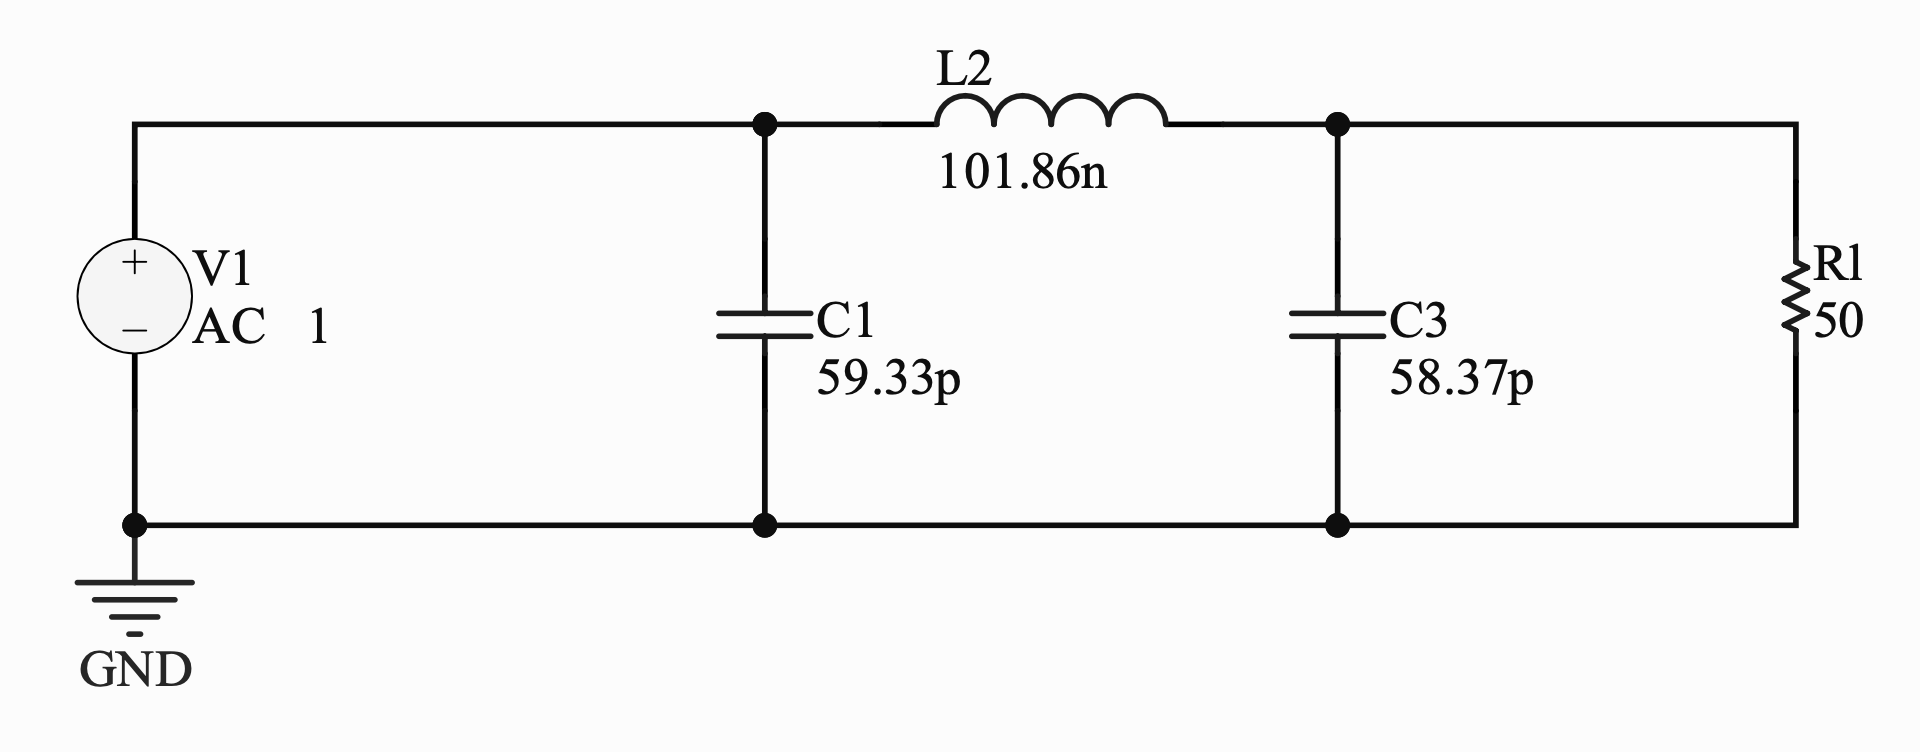
\includegraphics[width=\linewidth]{figures/2.ideal_components}
        \caption{Ideal Components}
    \end{subfigure}

    \medskip

    \begin{subfigure}[t]{0.8\textwidth}
        \centering
        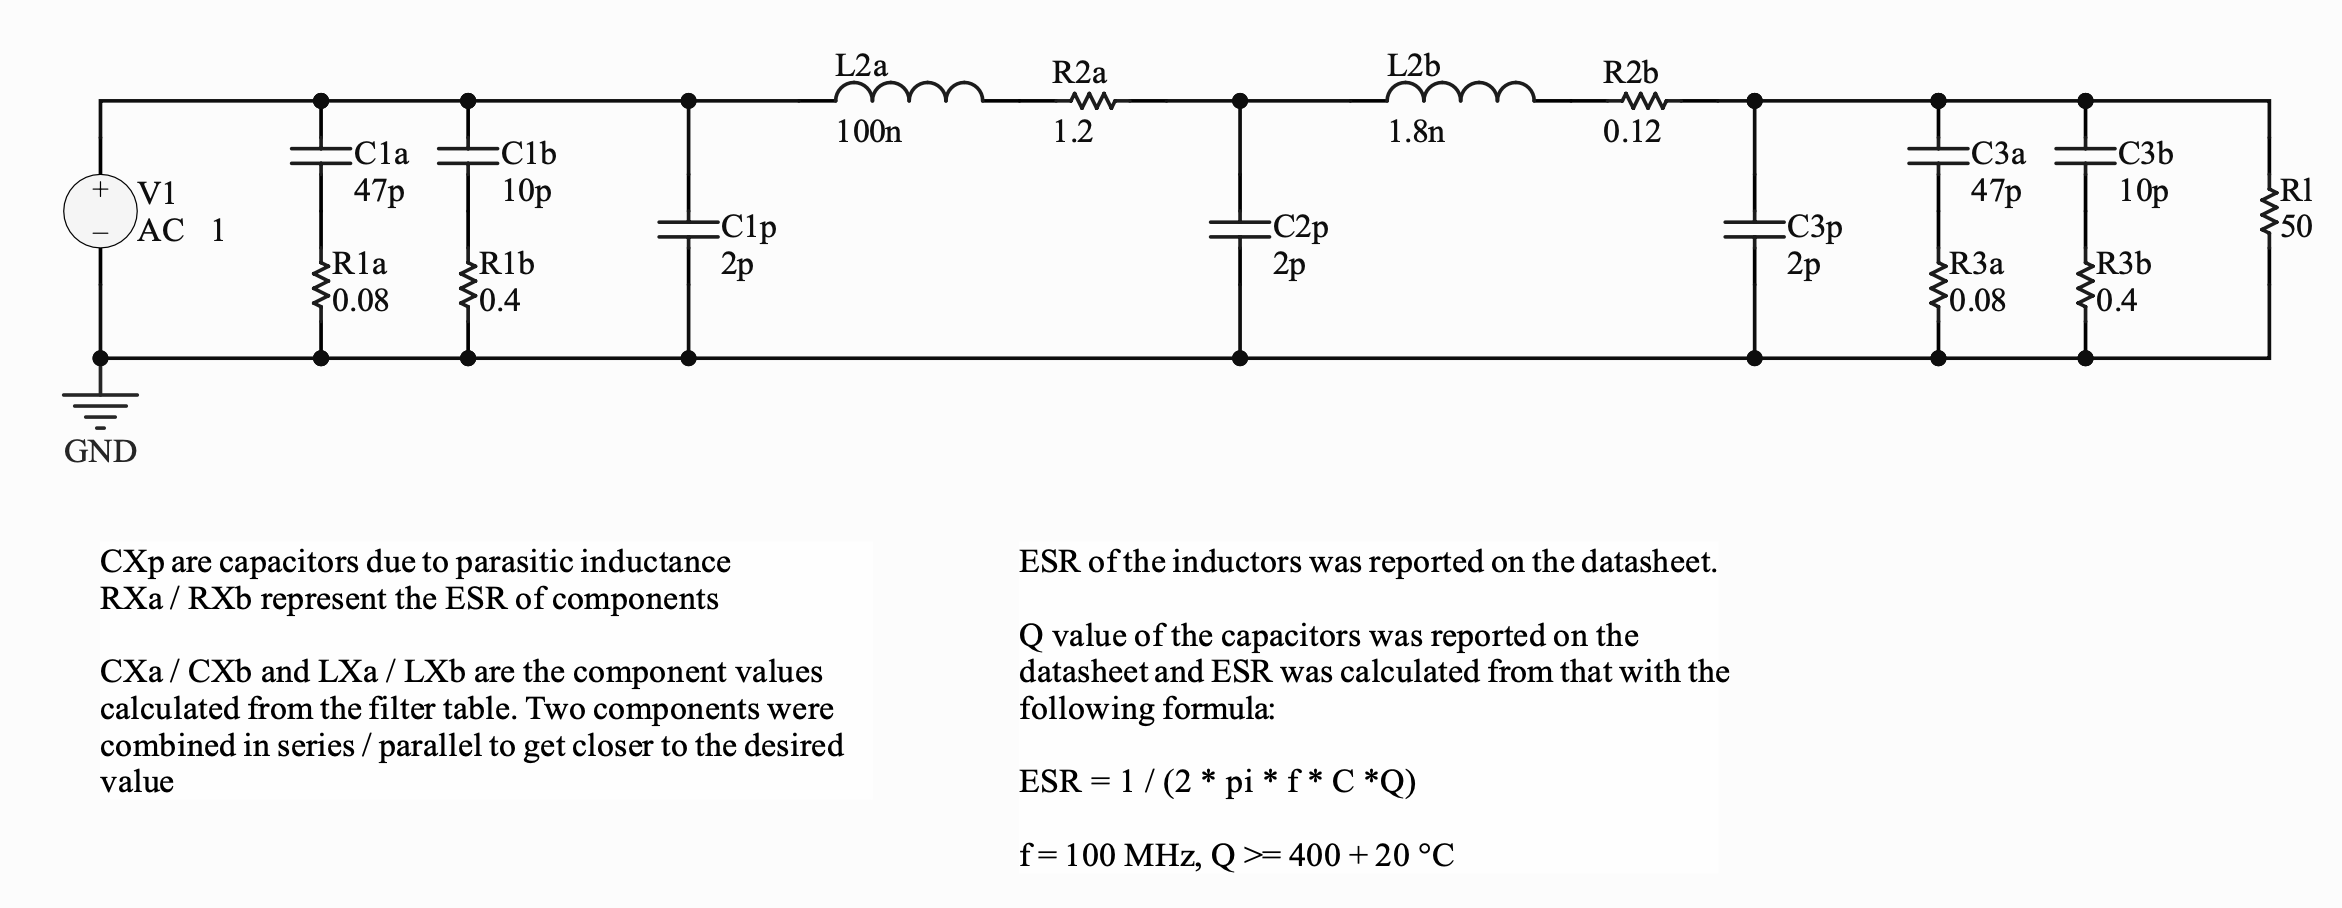
\includegraphics[width=\linewidth]{figures/2.real_components}
        \caption{Real Components}
    \end{subfigure}

    \medskip

    \begin{subfigure}[t]{0.8\textwidth}
        \centering
        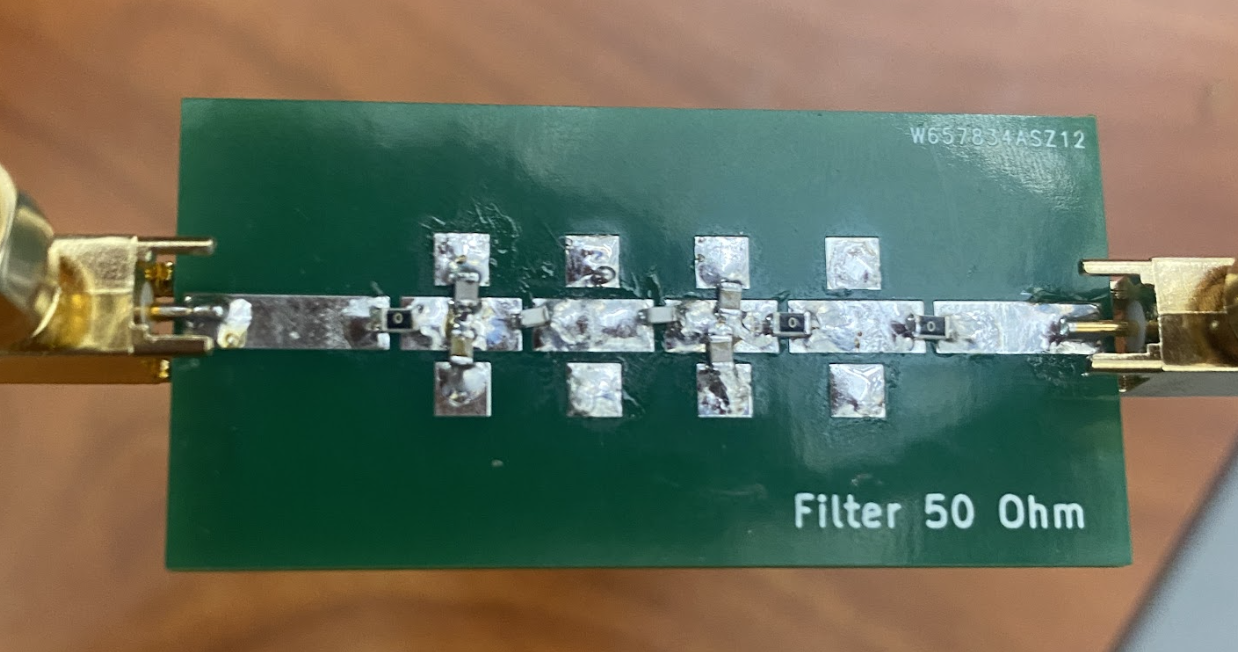
\includegraphics[width=\linewidth]{figures/2.assembled}
        \caption{Assembled Design}
    \end{subfigure}
\end{figure}

\newpage
\section{Hand Calculations}
% 1-2 pages of hand calculations and tables showing the following.  You may include source code here if it is extremely legible.  You may not just paste a spreadsheet here, but you can include it as a supplementary file for the report.
% •	How you picked your filter type and order including showing
%     o	Your in-band ripple is achievable by your design 
%     o	Your stop-band rejection is achievable by your design
%     o	For Butterworth filters: how you found wp for an in-band ripple of 1dB
% •	The filter table you used (include a citation showing where you found it)
% •	How you synthesized the ideal simulation components using your filter table
% •	Calculation showing power delivered to a 50 Ohm if your filter were driven by a 1Vpp, 0VDC offset, 50 MHz sine wave from a voltage source w/ 50 Ohm output impedance.  You will need your measured insertion loss to complete this calculation, and you may refer to the page in your report where I can check it.
We want to design an LC lowpass filter with an $f_c$ of 100 MHz and minimum attenuation of 20 dB at 200 MHz. The allowable passband ripple is 1 dB and the maximum insertion loss is 3 dB. The source and load resistance are equal at 50 ohms. \\
\\
We can then normalize the attenuation requirements to use attenuation curves:
\begin{align*}
    \frac{f}{f_c} = \frac{200 \text{ MHz}}{100 \text{ MHz}} = 2
\end{align*}
Now we want to select a normalized lowpass filter that offers at least 20 dB of attenuation at a ratio of $f/f_c = 2$.
\begin{figure}[H] 
    \centering 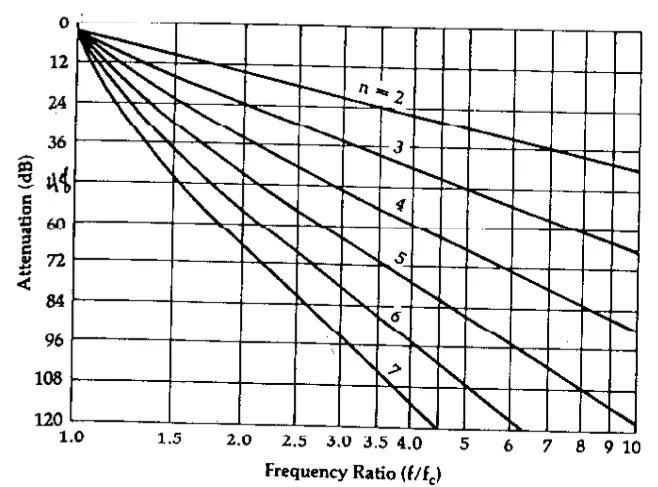
\includegraphics[width=0.5\columnwidth]{figures/3.attenuation_characteristics}
    \caption{
            \label{fig:2.attenuation_characteristics}
            Attenuation characteristics for a Chebyshev filter with 0.5-dB ripple.
    }
\end{figure}
\noindent
From the attenuation plot, we can see that a 3rd order chebyshev filter has greater than the required attenuation at $f/f_c=2$
% and that the attenuation is equal to 20 dB at $f/f_c \approx 1.7 \implies f_\text{stop band}=170 \text{ MHz}$.
Extracting the point at which there is 20 dB of rejection from the transfer function numerically, we get $f_\text{stop band}=170 \text{ MHz}$. \\
\\
We have chosen to use the 0.5 dB attenuation table, so the expected in band ripple is 0.5 dB.
At the desired stop band, $f = 200 \text{ MHz} \to f/f_c=2$, we can see that there is 24 dB of attenuation.\\
\\
We can predict the attenuation as a function of frequency using
\begin{align*}
    A_\text{dB}=10\log\left[1+\epsilon^2C_n^2\left(\frac{\omega}{\omega_c}\right)'\right]
\end{align*}
Where:
\begin{enumerate}
  \item $\epsilon=\sqrt{10^{R_\text{dB}/10}-1} = 0.3493$ ($R_{dB}$ = 1 dB is the allowable passband ripple)
  \item $\left(\frac{\omega}{\omega_c}\right)' = \left(\frac{\omega}{\omega_c}\right) \cosh B$
  \item $B=\frac{1}{n}\cosh^{-1}\left(\frac{1}{\epsilon}\right)$
  \item $C_3(x)=4x^3-3x$
\end{enumerate}
% Plotting this in python (\href{https://github.com/kavidey/e157/blob/main/dp_01/predict_chebyshev.py}{code link}) we get:
% \begin{figure}[ht] 
%     \centering 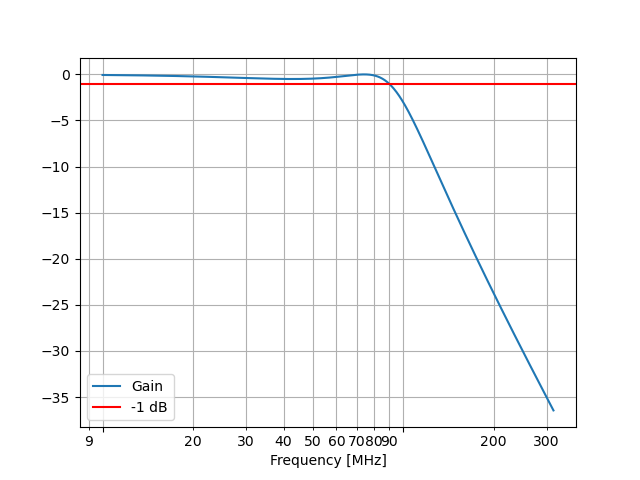
\includegraphics[width=0.5\columnwidth]{figures/3.mag}
%     \caption{
%             \label{fig:2.mag}
%             Attenuation characteristics for a Chebyshev filter with 0.5-dB ripple.
%     }
% \end{figure}
% Extracting the pass band ripple from the graph we get 0.5 dB, as predicted from the filter table in figure \ref{fig:2.filter_table}
The following table can be used to calculate component values for $n=3$ and $R_S/R_L = 1$ as follows:
\begin{figure}[H] 
    \centering 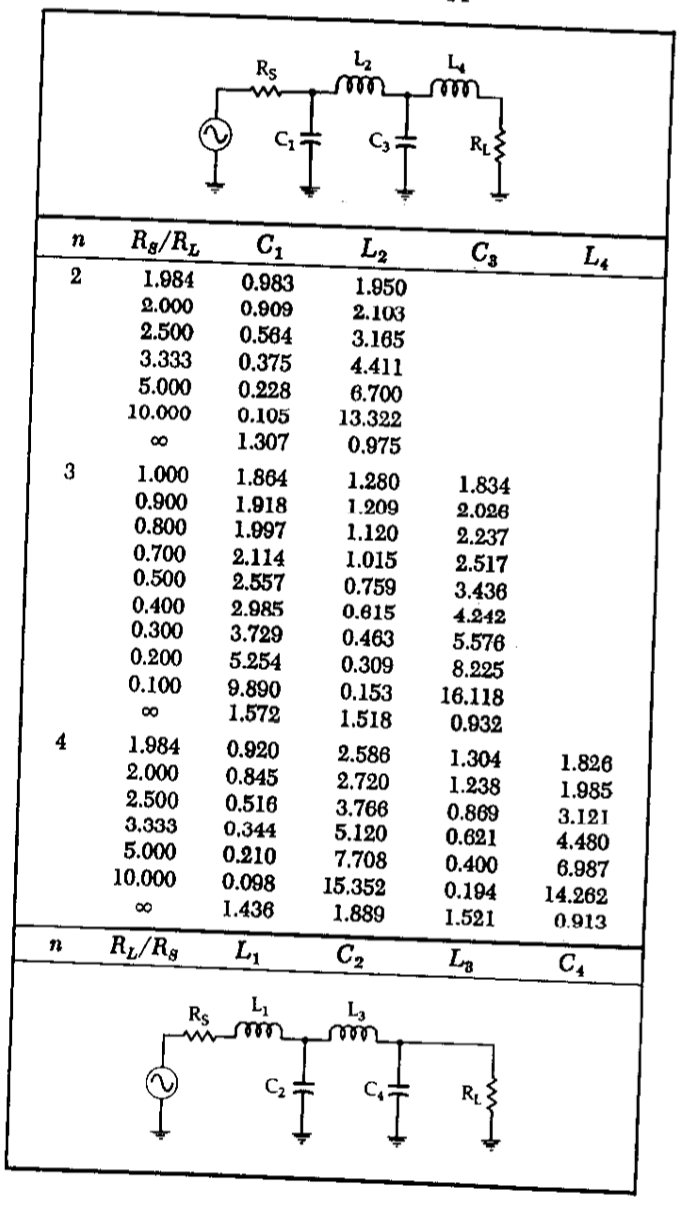
\includegraphics[width=0.3\columnwidth]{figures/3.filter_table}
    \caption{
            \label{fig:2.filter_table}
            Chebyshev Low-Pass Prototype Element Values for 0.5-dB Ripple.
    }
\end{figure}
\noindent
Plugging in we get:
\begin{align*}
    C_1 = \frac{1.864}{2\pi(100\times10^6)50} = 59.33 \text{ pF} \\
    L_2 = \frac{(1.280)(50)}{2\pi(100\times10^6)} = 101.86 \text{ nH} \\
    C_3 = \frac{1.834}{2\pi(100\times10^6)50} = 58.37 \text{ pF}
\end{align*}
Because we are making a lowpass filter, we can use the provided schematic as is. We have chosen to use the \textbf{top} schematic in \ref{fig:2.filter_table}. \\
\\
Calculation showing power delivered to a 50 Ohm if your filter were driven by a 1 Vpp, 0 VDC offset, 50 MHz sine wave from a voltage source w/ 50 Ohm output impedance.\\
\\
The input wave has a power of
$$P=\left(\frac{1 \ V}{2\sqrt{2}}\right)^2 \frac{1}{50 \Omega} = 2.5 \text{ mW} \approx 4 \text{ dBm}$$
50 MHz is a low enough frequency that we can assume the only loss is due to insertion loss (see page \pageref{sec:s21_dcstop} for insertion loss measurement).
Then the total power delivered into the load is:
$$4 \text{ dBm} - \text{Insertion Loss} = 4 \text{ dBm} - 0.84 \text{ dBm} = 3.16 \text{ dBm} \approx 2 \text{ mW} $$

\newpage
\section{Magnitude of S21 in Pass band}
% Magnitude of S21 in your pass band for all four designs
% •	Use the frequency range 40MHz-130MHz.  Display in on a linear scale.
% •	Use dB as your y-axis units
% •	Do not overlay these graphs.  Please include four of them in a 2x2 grid.
% •	Each representation needs to include annotated markers that show the magnitude and frequency of 
%     o	The maximum value in the pass band
%     o	The minimum ripple value in the pass band
%     o	The pass band edge. (In a Butterworth or Chebyshev II filter, this might be the same marker as the minimum ripple value.)
\begin{figure}[H]
    \begin{subfigure}[t]{.49\textwidth}
      \centering
      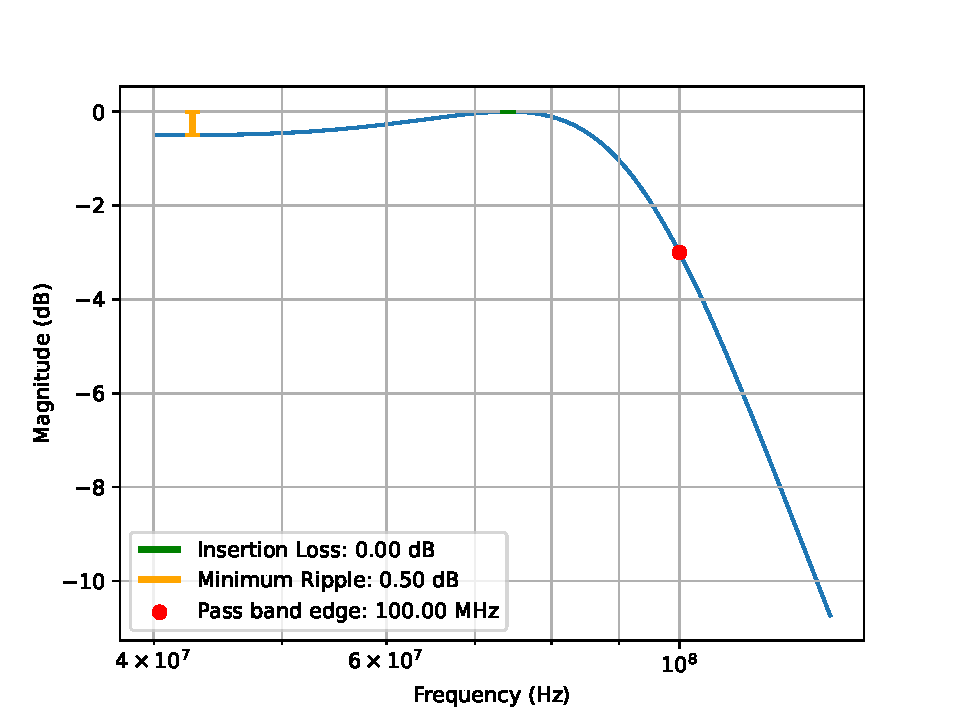
\includegraphics[width=\linewidth]{figures/4.analytical}
      \caption{Analytical Design}
    \end{subfigure}
    \hfill
    \begin{subfigure}[t]{.49\textwidth}
      \centering
      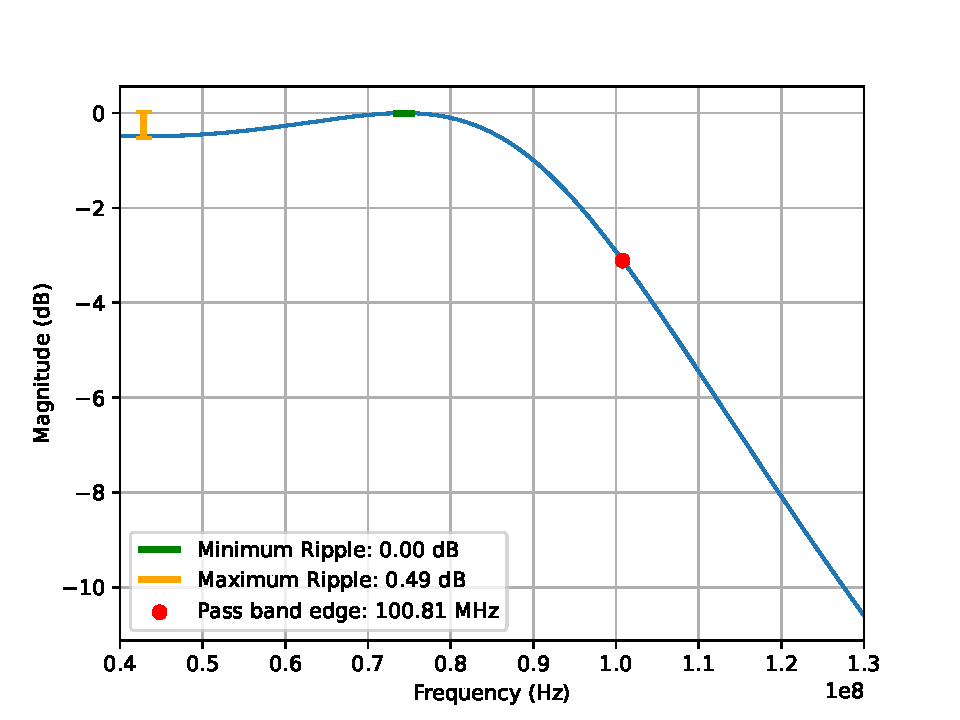
\includegraphics[width=\linewidth]{figures/4.ideal}
      \caption{Simulated design with ideal components}
    \end{subfigure}
  
    \medskip
  
    \begin{subfigure}[t]{.49\textwidth}
      \centering
      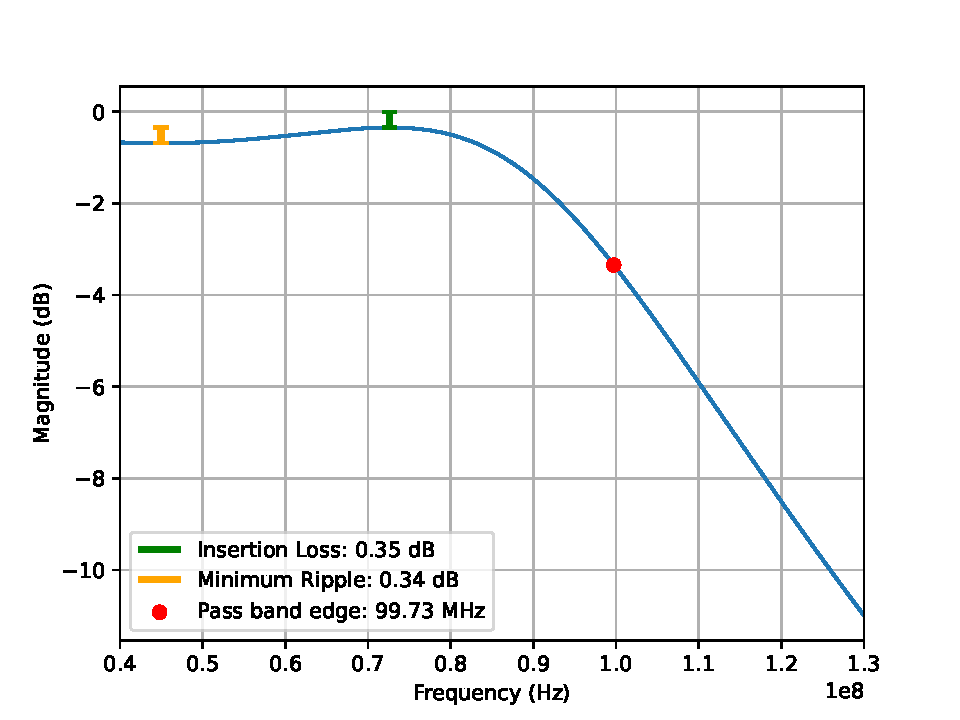
\includegraphics[width=\linewidth]{figures/4.real}
      \caption{Simulated Design with real components}
    \end{subfigure}
    \hfill
    \begin{subfigure}[t]{.49\textwidth}
      \centering
      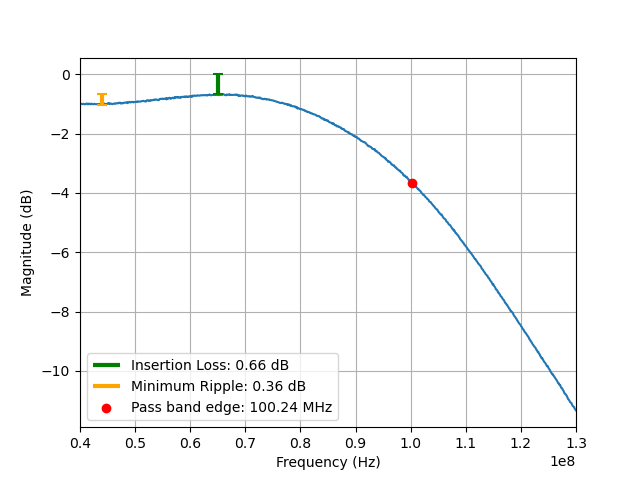
\includegraphics[width=\linewidth]{figures/4.assembled}
      \caption{Assembled Design}
    \end{subfigure}
  \end{figure}

\newpage
\section{Phase of S21 in Pass band}
% Phase of S21 in your pass band for three designs: the ideal simulation, the real simulation and the measured design.
% •	Use the frequency range 40MHz-130MHz.  Display in on a linear scale.
% •	Use degrees between -180/+180 as your y-axis units (i.e.: provide a wrapped phase plot)
% •	Overlay these graphs on one frequency axis.
% •	Each representation needs to include one annotated marker at the band edge (which you found from your magnitude plot) that shows the phase and frequency.
\begin{figure}[H]
    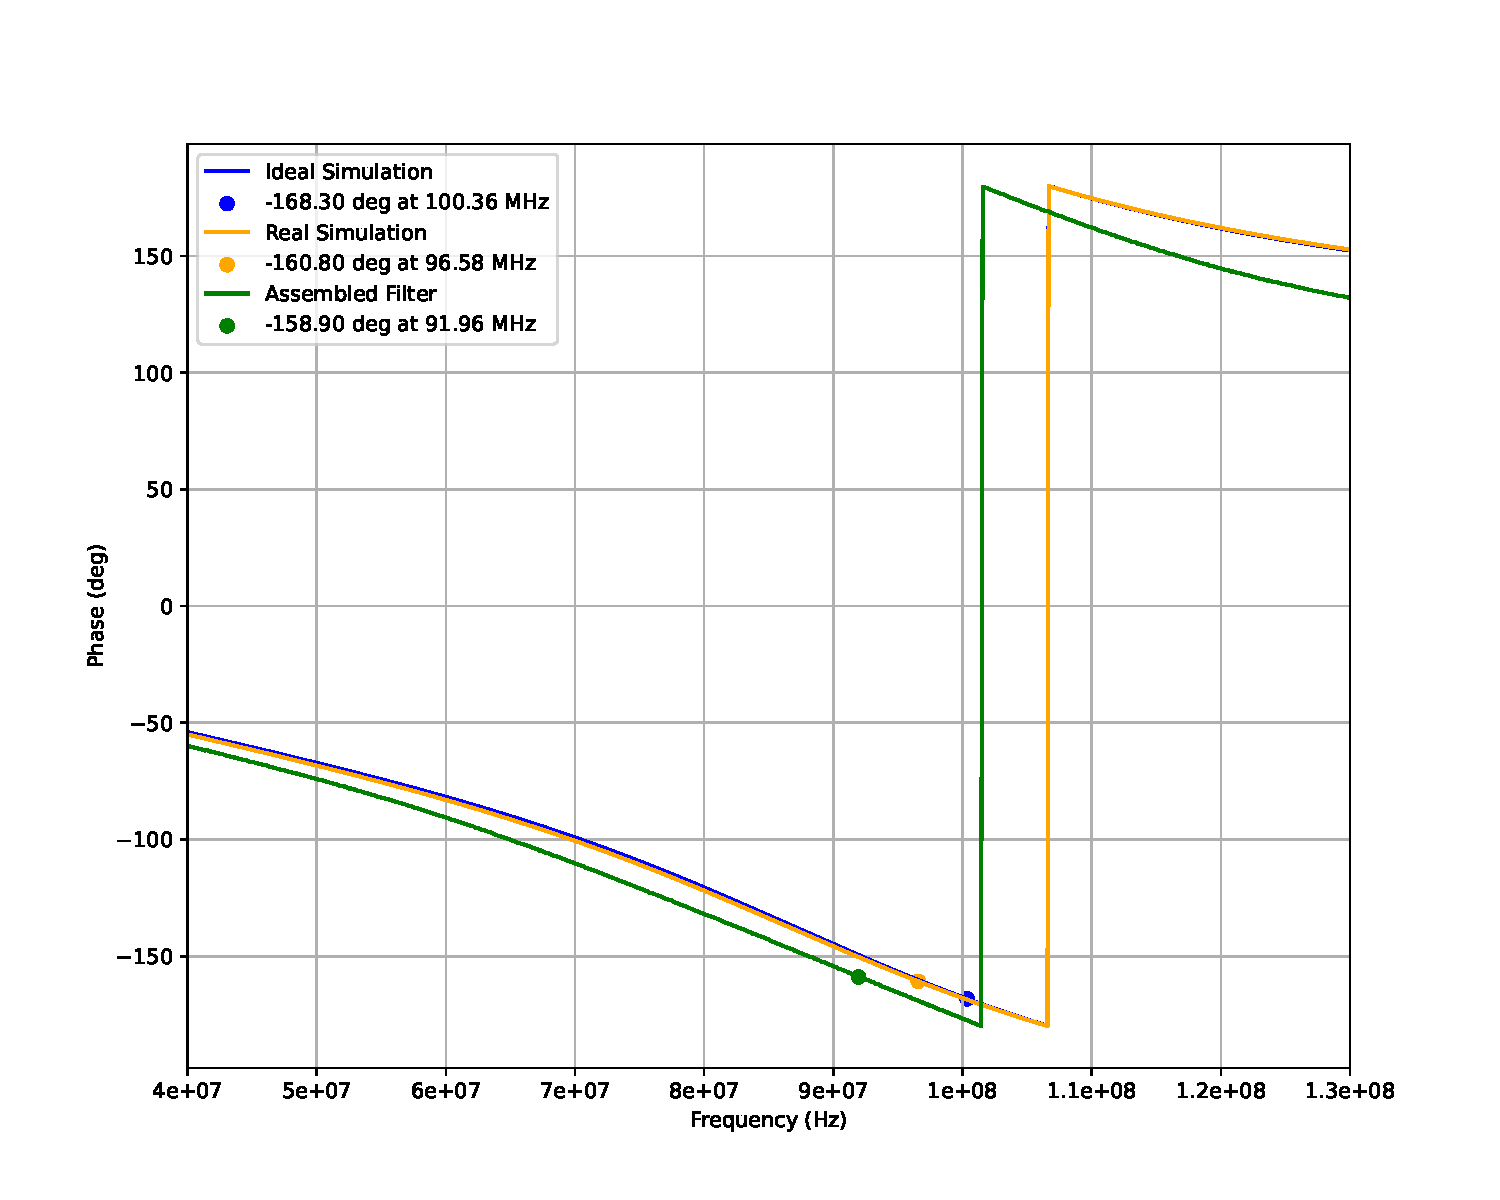
\includegraphics[width=\linewidth]{figures/5.phase}
    \caption{Phase of S21 in Pass band for ideal simulation, real simulation, and assembled design}
\end{figure}

\newpage
\section{Magnitude of S21 from DC to Stop band} \label{sec:s21_dcstop}
% Magnitude of S21 from DC to your stop band for all four designs
% •	Use the frequency range 0Hz to 300MHz (or as low as the instrument will go for measurements).  Display your frequency range on a log scale.
% •	Use dB as your y-axis units.
% •	Do not overlay these graphs.  Please include four of them in a 2x2 grid.
% •	Each representation needs to include annotated markers that show the magnitude and frequency of 
%     o	The value of insertion loss in the pass band (i.e.: the “DC” value of S21)
%     o	The pass band edge
%     o	The stop band edge.
\begin{figure}[H]
    \begin{subfigure}[t]{.49\textwidth}
      \centering
      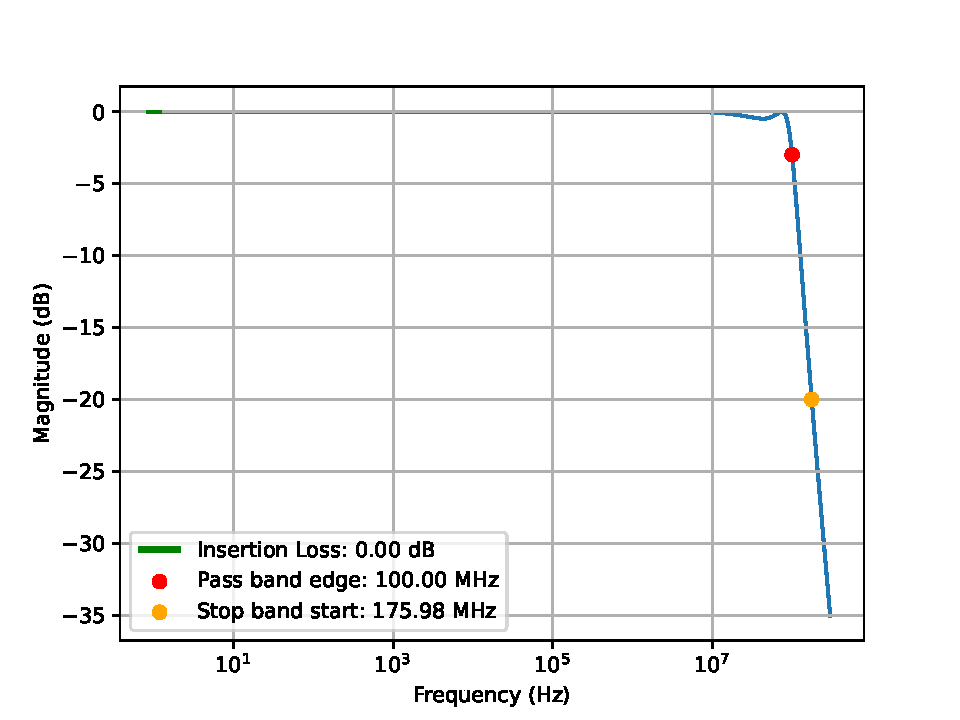
\includegraphics[width=\linewidth]{figures/6.analytical.pdf}
      \caption{Analytical Design}
    \end{subfigure}
    \hfill
    \begin{subfigure}[t]{.49\textwidth}
      \centering
      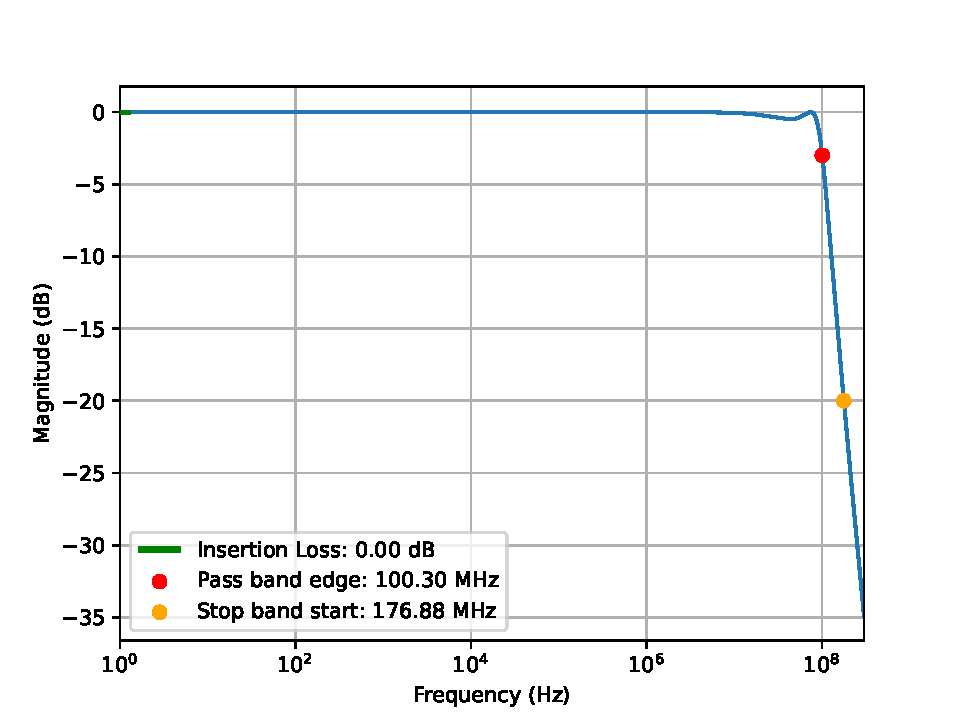
\includegraphics[width=\linewidth]{figures/6.ideal}
      \caption{Simulated design with ideal components}
    \end{subfigure}
  
    \medskip
  
    \begin{subfigure}[t]{.49\textwidth}
      \centering
      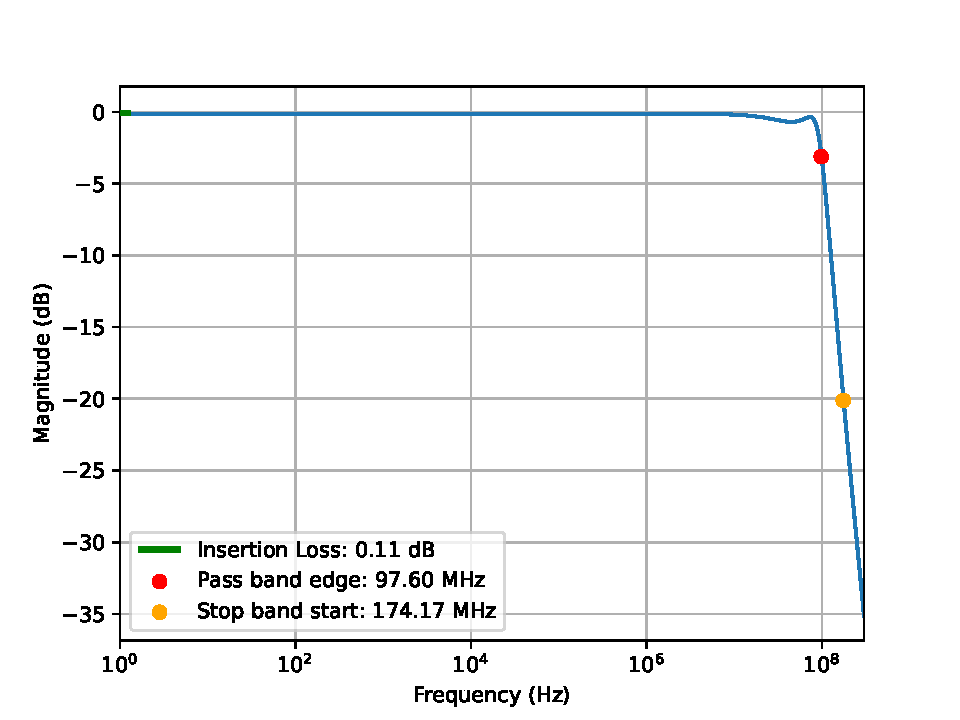
\includegraphics[width=\linewidth]{figures/6.real}
      \caption{Simulated Design with real components}
    \end{subfigure}
    \hfill
    \begin{subfigure}[t]{.49\textwidth}
      \centering
      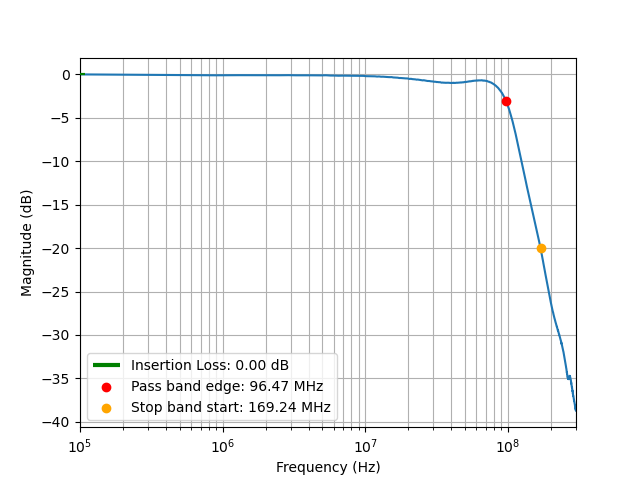
\includegraphics[width=\linewidth]{figures/6.assembled}
      \caption{Assembled Design}
    \end{subfigure}
  \end{figure}

\newpage
\section{Magnitude of S11 from DC to Stop band}
% Magnitude of S11 from DC to your stop band for all four designs.  Note that for the analytical design you will need to derive this from your S21 magnitude and power conservation.
% •	Use the frequency range 0Hz to 300MHz (or as low as the instrument will go for measurements).  Display your frequency range on a log scale.
% •	Use dB as your y-axis units.
% •	Do not overlay these graphs.  Please include four of them in a 2x2 grid.
% •	Each representation needs to include annotated markers that show the magnitude and frequency of 
%     o	The pass band edge
%     o	The stop band edge.
\begin{figure}[H]
    \begin{subfigure}[t]{.49\textwidth}
      \centering
      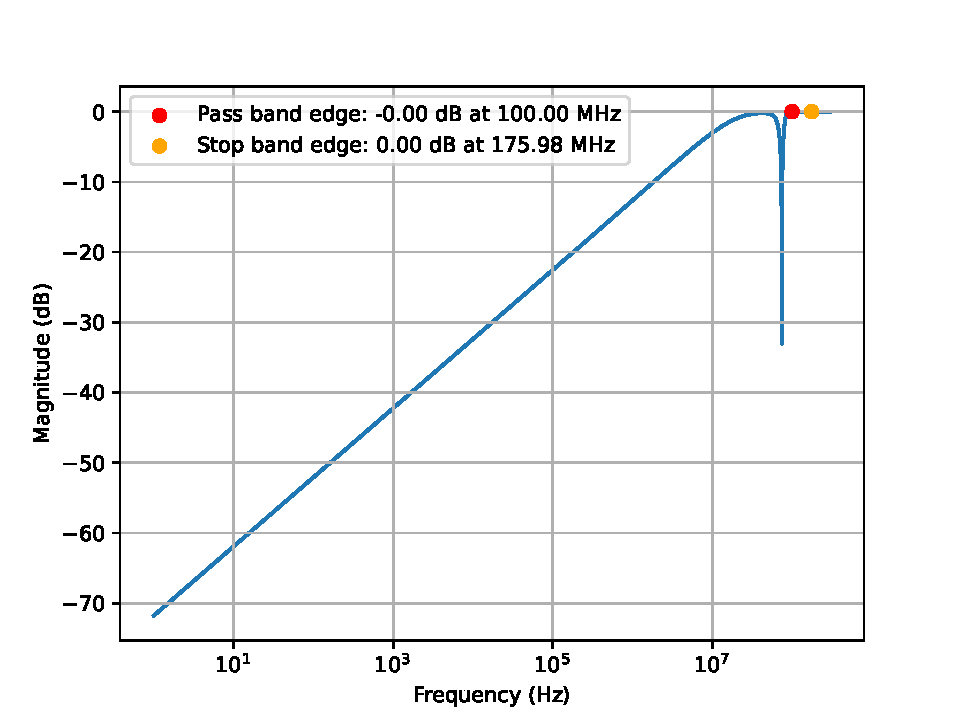
\includegraphics[width=\linewidth]{figures/7.analytical}
      \caption{Analytical Design}
    \end{subfigure}
    \hfill
    \begin{subfigure}[t]{.49\textwidth}
      \centering
      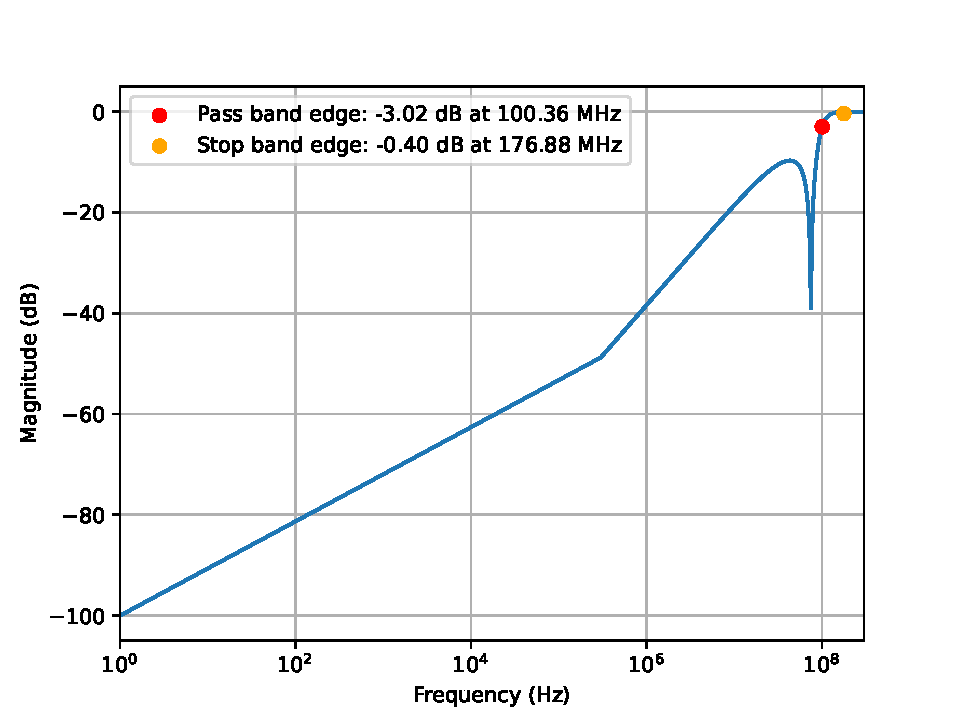
\includegraphics[width=\linewidth]{figures/7.ideal}
      \caption{Simulated design with ideal components}
    \end{subfigure}
  
    \medskip
  
    \begin{subfigure}[t]{.49\textwidth}
      \centering
      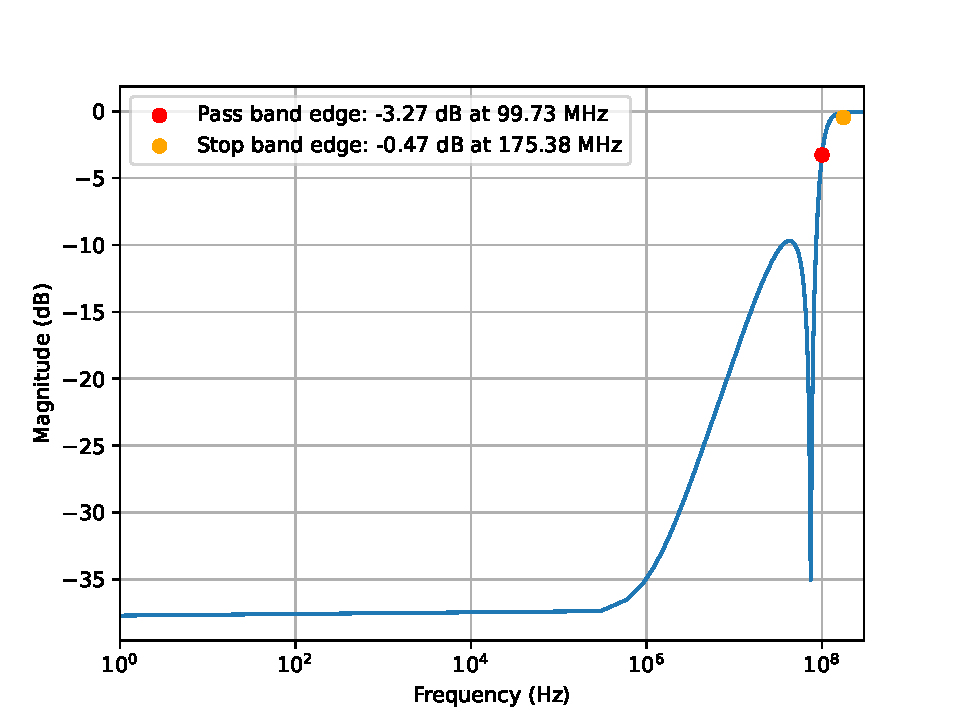
\includegraphics[width=\linewidth]{figures/7.real}
      \caption{Simulated Design with real components}
    \end{subfigure}
    \hfill
    \begin{subfigure}[t]{.49\textwidth}
      \centering
      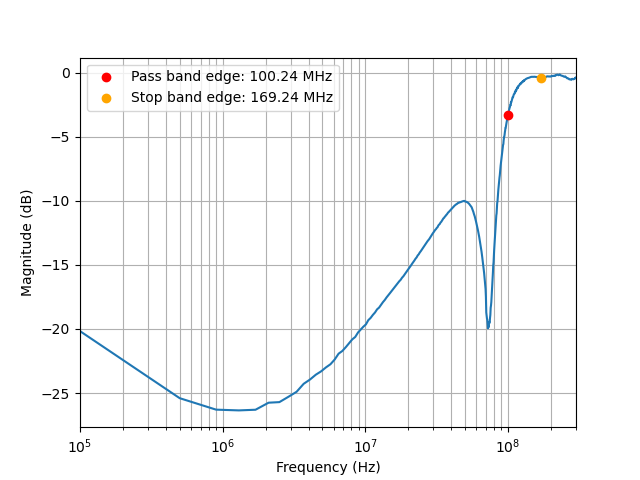
\includegraphics[width=\linewidth]{figures/7.assembled}
      \caption{Assembled Design}
    \end{subfigure}
  \end{figure}

\newpage
\section{Smith Charts for S11 and S21 from DC to Stop band}
% Smith Charts for S11 and S21 from DC to your stop band for three designs: the ideal simulation, the real simulation and the measured results.  Use the frequency range 0Hz to 300MHz and do not overlay the graphs, instead arranging them in a 3x2 grid with S11 on the left.
\begin{figure}[H]
    \begin{subfigure}[t]{.49\textwidth}
        \centering
        S11
    \end{subfigure}
    \hfill
    \begin{subfigure}[t]{.49\textwidth}
        \centering
        S21
    \end{subfigure}

    \medskip
    
    \begin{subfigure}[t]{.49\textwidth}
      \centering
      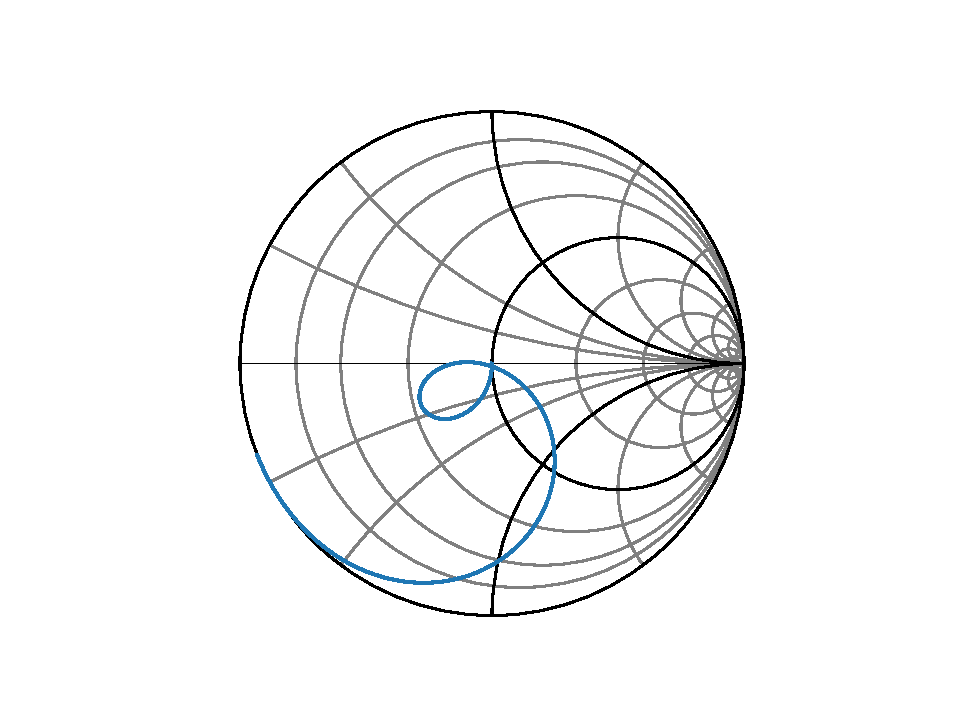
\includegraphics[width=\linewidth]{figures/8.s11.ideal}
      \caption{Ideal Simulation S11}
    \end{subfigure}
    \hfill
    \begin{subfigure}[t]{.49\textwidth}
      \centering
      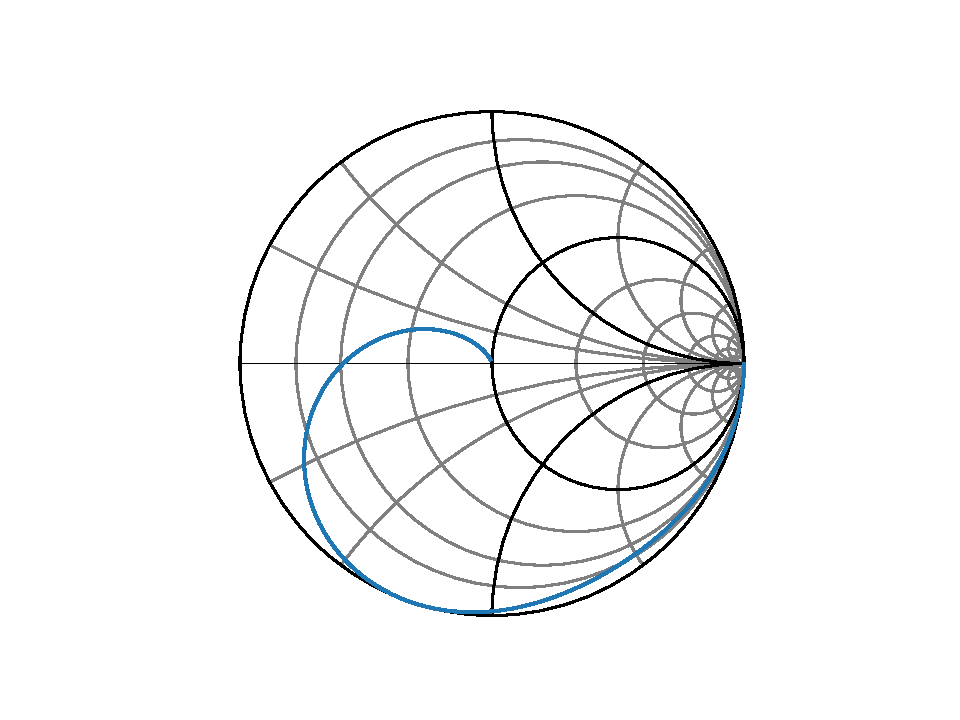
\includegraphics[width=\linewidth]{figures/8.s21.ideal}
      \caption{Ideal Simulation S21}
    \end{subfigure}

    \medskip
    
    \begin{subfigure}[t]{.49\textwidth}
      \centering
      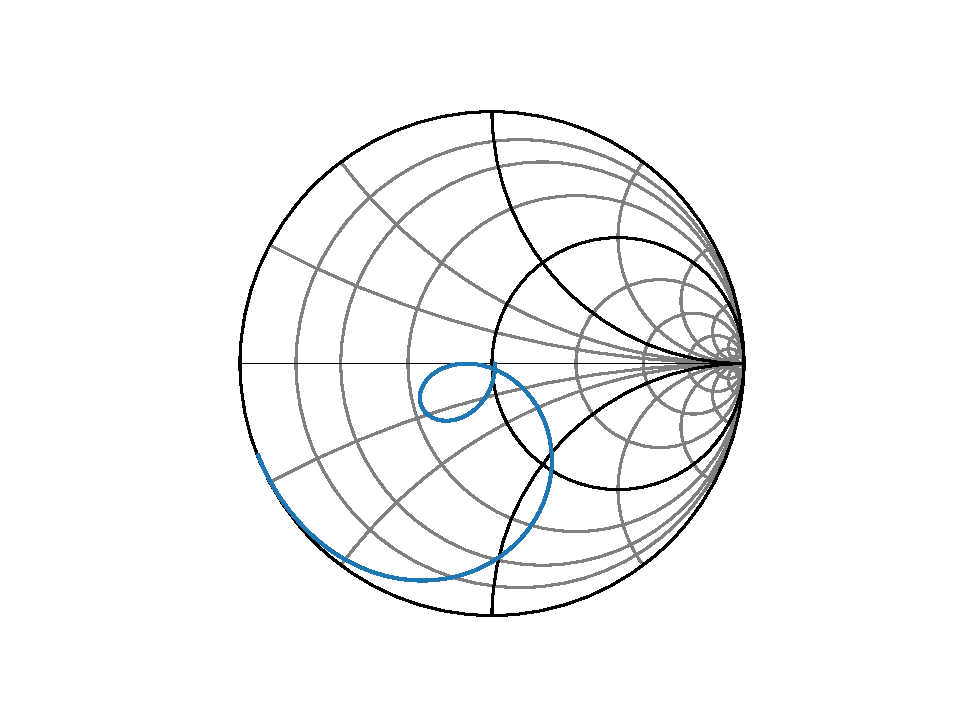
\includegraphics[width=\linewidth]{figures/8.s11.real}
      \caption{Real Simulation S11}
    \end{subfigure}
    \hfill
    \begin{subfigure}[t]{.49\textwidth}
      \centering
      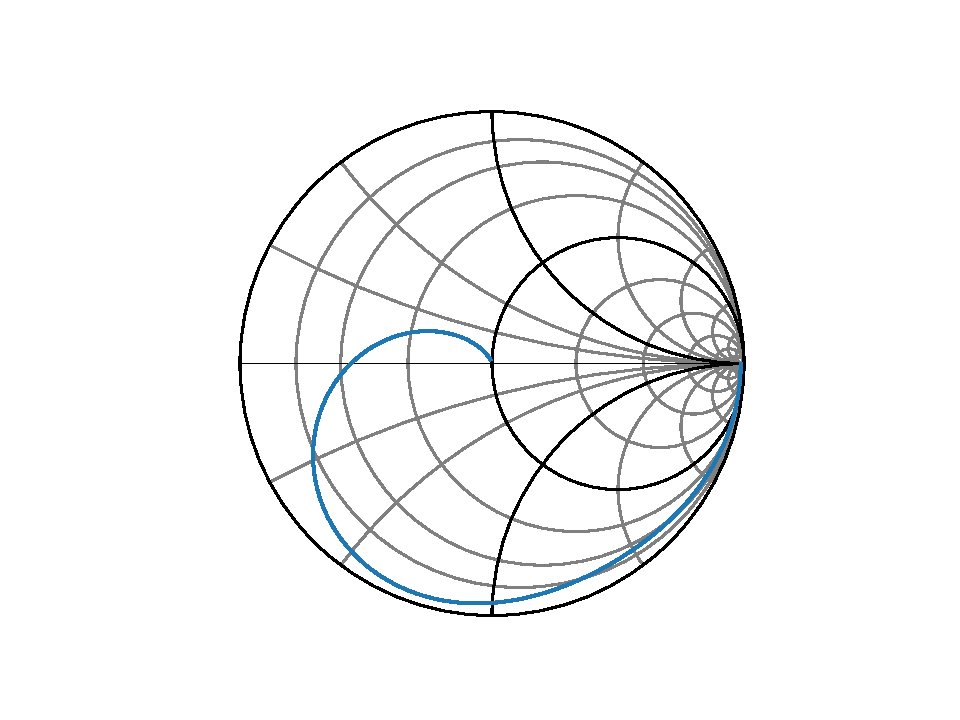
\includegraphics[width=\linewidth]{figures/8.s21.real}
      \caption{Real Simulation S21}
    \end{subfigure}
  
    \medskip
  
    \begin{subfigure}[t]{.49\textwidth}
      \centering
      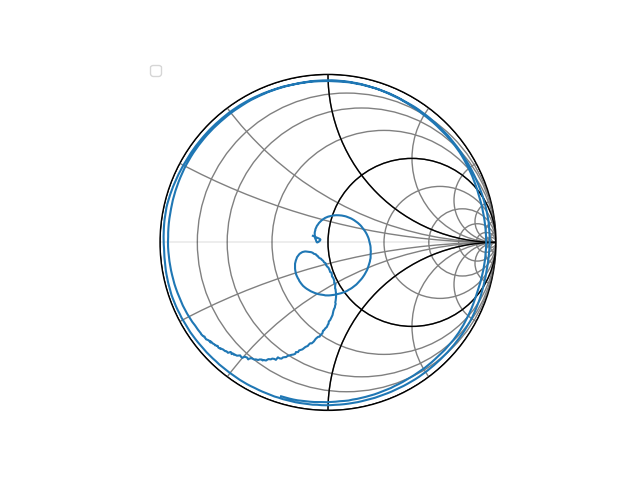
\includegraphics[width=\linewidth]{figures/8.s11.assembled}
      \caption{Assembled Design S11}
    \end{subfigure}
    \hfill
    \begin{subfigure}[t]{.49\textwidth}
      \centering
      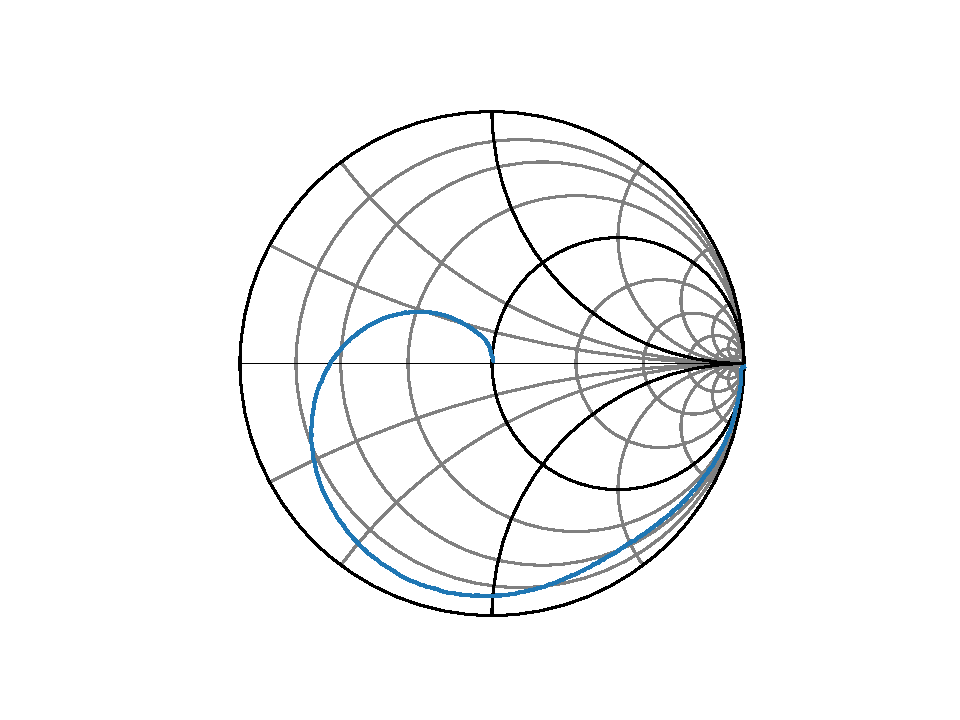
\includegraphics[width=\linewidth]{figures/8.s21.assembled}
      \caption{Assembled Design S21}
    \end{subfigure}
\end{figure}

\newpage
\section{Discussions}
% Discussion of discrepancies between analytical, simulated and measured results.  Quantitatively justify differences between them, including any modifications you made to your models to make your simulations match your measurements better (e.g.: board parasitics).  Refer to prior figures in your report for supporting evidence in this discussion.
% Issue: the table assumed that we wanted the corner frequency to be at -3db, not -1db as the filter specs say.
% Inspecting the analytical Chebyshev 1 attenuation plot, we find that we would need to adjust f_c from 100 MHz to 111.5 MHz for the attenuation to be 1db at 100 MHz. This would result in a stop band edge of 196.1 MHz, which is still within the desired filter parameters.
\newpage
\section{Takeaways}
% One paragraph about one thing you learned about RF design doing this project.

% referencing bibliography
% ~\cite{melissinos, Cyr, Wiki}

% figures
% \begin{figure}[ht] 
%     \centering \includegraphics[width=0.8\columnwidth]{sr_setup}
%     \caption{
%             \label{fig:samplesetup}
%             Every figure MUST have a caption.
%     }
% \end{figure}

% equations
% \begin{equation} \label{eq:aperp} % the label is used to reference the equation
%     u(\lambda,T)=\frac{8\pi hc\lambda^{-5}}{e^{hc/\lambda kT}-1},
% \end{equation}
%
% ~\ref{fig:samplesetup}

% tables
% \begin{table}[ht]
%     \begin{center}
%         \caption{Every table needs a caption.}
%         \label{tbl:bins} % spaces are big no-no withing labels
%         \begin{tabular}{|cc|}
%             \hline
%             \multicolumn{1}{|c}{$x$ (m)} & \multicolumn{1}{c|}{$V$ (V)} \\
%             \hline
%             0.0044151                    & 0.0030871                    \\
%             0.0021633                    & 0.0021343                    \\
%             0.0003600                    & 0.0018642                    \\
%             0.0023831                    & 0.0013287                    \\
%             \hline
%         \end{tabular}
%     \end{center}
% \end{table}
%
% Table~\ref{tbl:bins} is an example.

% \newpage

% bibliography
% \begin{thebibliography}{99}
%     \bibitem{levitator_paper}
%     Asier Marzo, Adrian Barnes, Bruce W. Drinkwater; TinyLev: A multi-emitter single-axis acoustic levitator. \textit{Rev. Sci. Instrum.} 1 August 2017; 88 (8): 085105. \href{https://doi.org/10.1063/1.4989995}{https://doi.org/10.1063/1.4989995}

%     \bibitem{levitator_instructions}
%     Instructables ultrasonic levitator materials and instructions. \href{https://www.instructables.com/Acoustic-Levitator/}{https://www.instructables.com/Acoustic-Levitator/}
% \end{thebibliography}
\end{document}